\section{Estágio de execução}
	\subsection{Diagrama de Classe}
  \begin{figure}[h]
    \begin{center}
	\begin{tikzpicture}
	\umlclass[x=0,y=0]{EX}{
	+ clock : input bit \\
	+ pcInput : input bit[32] \\ 
	+ pcWrite : input bit \\
	+ pcOutput : output bit[32] \\
	+ instruction : output bit[32] \\}			
	{}
	\end{tikzpicture}
\end{center}
  \end{figure}
		
		\subsection{Definições de entrada e saída}
		
	\begin{center}
		\begin{longtable}[pos]{| l | c | c | m{7cm} |} \hline
			\multicolumn{1}{|c|}{\cellcolor[gray]{0.9}\textbf{Nome}} & 
			\multicolumn{1}{c|}{\cellcolor[gray]{0.9}\textbf{Tamanho}} & 
			\multicolumn{1}{c|}{\cellcolor[gray]{0.9}\textbf{Direção}} &
			\multicolumn{1}{c|}{\cellcolor[gray]{0.9}\textbf{Descrição}} \\ \hline
			\endhead
			\hline
			\endlastfoot
			
			data\_a & 32 & Entrada & Dado do primeiro operando. \\ \hline
			data\_b & 32 & Entrada & Dado do segundo operando. \\ \hline
			pc\_in & 32 & Entrada & Valor do PC atual. \\ \hline
			orig\_pc & 2 & Define qual a origem do próximo pc, ou seja, se é branch, jump ou a próxima instrução \\ \hline
			
			
			
			
		\end{longtable}
	\end{center}
	
	\subsection{Datapath Interno}
	
	\begin{figure}[ht]
		\begin{center}
		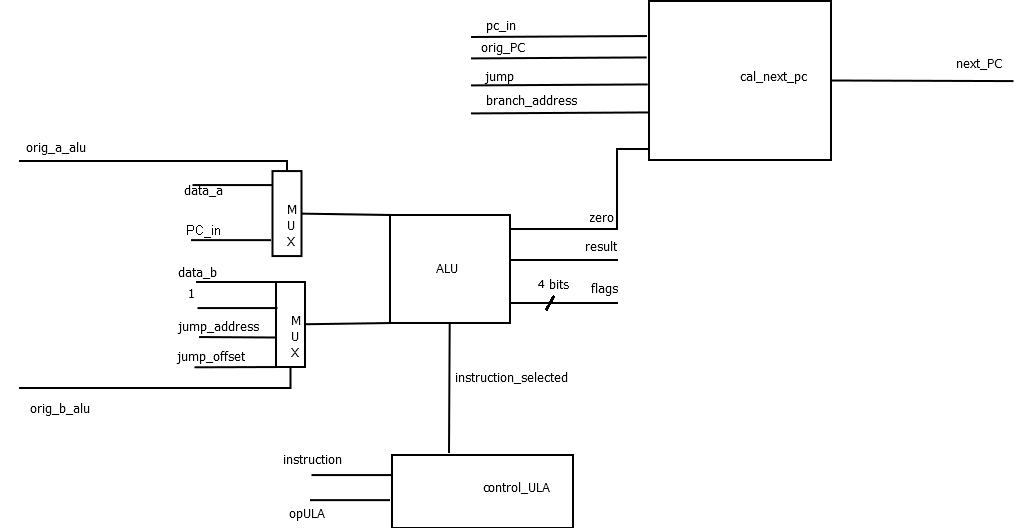
\includegraphics[scale = 0.5]{./datapath/step3.png}
		\caption*{Datapath interno do estágio de execução (EX).}
		\end{center}
	\end{figure}
